\chapter{Temps de diffusion élastique}
\label{ch:TauS_PRL}

Dans les chapitres précédents, nous avons détaillé comment était produite notre onde de matière, et plus particulièrement l'utilisation de techniques de refroidissement à l'extrême nous permettant d'obtenir un condensat de Bose-Einstein assimilable à une onde plane $\etat{\mathbf{k}=0}$. Nous avons aussi discuté comment est généré notre désordre optique et nous nous sommes focalisés sur ses propriétés statistiques et spatiales.

À présent, nous allons nous concentrer sur la mesure directe du temps de diffusion élastique $\taus$, lié au déphasage de l'onde lors d'une collision dans le désordre. Cette mesure directe demande des efforts expérimentaux conséquents dans le domaine de la matière condensée (les propriétés de transport découlent du temps de transport $\taub$), mais celle-ci reste aisée en optique (décroissance balistique d'un faisceau laser) ainsi qu'à l'aide d'atomes ultra-froids (suivi de l'état initial). De nombreuses méthodes ont ainsi été développées, telles que des techniques de microscopie \citep{jacques2012reflectance}\citep{martin2016determination}, des mesures de corrélation pour des ondes classiques \citep{sebbah2002spatial}\citep{hildebrand2014observation}\citep{obermann2014measuring}, des transmissions balistiques \citep{page1996group}\citep{savo2017observation} ou encore des oscillations de Shubnikov-de Haas de la magnéto-conductivité dans des systèmes électroniques \citep{niederer1974magneto}\citep{bockelmann1990single}\citep{monteverde2010transport}. Cependant, des comparaisons quantitatives à des théories ou des simulations restent rares.




La détermination expérimentale du temps de diffusion élastique a été réalisée en 2015 lors de la thèse de Jérémie Richard \citep{richard2015propagation}. Cependant, le traitement et l'exploitation de ces données expérimentales, leur comparaison à des simulations numériques, et l'orientation que nous avons donnée à ce projet constituent des travaux réalisés cours de ma thèse. Le temps de diffusion élastique $\taus$ a ainsi été étudié en fonction de l'amplitude du désordre $\VR$ et de l'énergie de l'onde (énergie cinétique, ou de manière équivalente son impulsion $k_{\mathrm{i}}$), permettant ainsi de suivre $\taus$ sur plus de trois ordres de grandeur. Nous avons ainsi pu explorer les régimes de diffusion faible et de diffusion forte, ainsi que la transition entre ces régimes que nous avons pu étudier quantitativement. Cela nous a plus particulièrement permis de discuter la pertinence du critère de Ioffe-Regel $k_{\mathrm{i}}\ls\sim 1 $ pour décrire cette transition. Les résultats de cette étude ont donné lieu à une publication dans la revue \emph{Physical Review Letters} \citep{richard2019elastic}.



\section{Approximation de Born}
Dans cette section, nous allons nous concentrer sur la description du temps de diffusion élastique dans le régime de désordre faible. Ce régime perturbatif, appelé \emph{régime de Born}, fournit une image intuitive de la physique du désordre et reste le seul régime permettant d'obtenir des résultats quantitatifs. Cette notion de régime perturbatif sera précisée formellement à l'aide d'un développement de la \emph{Self-energy} au cours du chapitre \ref{ch:TauS_NJP}.

\subsection{Temps de diffusion élastique dans le régime de désordre faible}
L'approximation de Born consiste à traiter l'effet du désordre $V(\mathbf{x})$ de manière perturbative\footnote{Une définition plus précise de l'approximation de Born basée sur le concept de \emph{Self-Energy} sera donnée dans le chapitre \ref{ch:TauS_NJP}.}.  Dans cette vision de désordre faible, on peut considérer la propagation dans le désordre comme une succession d'évènements de diffusion simple pour lesquels l'onde diffuse sur un diffuseur unique. L'étude du temps de diffusion élastique se concentre donc sur la dynamique d'un unique évènement de diffusion.



Dans le régime désordre faible, on peut considérer l'effet du désordre comme un couplage de l'état initial $\etat{\mathbf{k}_{\mathrm{i}}}$ à un continuum d'états d'impulsion $\etat{\mathbf{k}'}$ pour lesquels $\left| \mathbf{k}' \right| = \left| \mathbf{k}_{\mathrm{i}} \right| $ afin de satisfaire la conservation de l'énergie, les collisions étant élastiques. Cette situation est illustrée figure \ref{fig:illustration_contexte_taus}. 

\begin{figure}
\centering
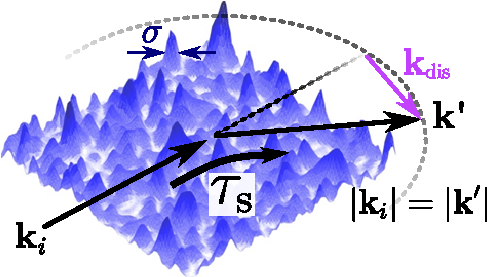
\includegraphics[scale=1]{Fig/TauS_PRL/illustration_contexte_taus.pdf}
\caption{\textbf{Illustration du temps de diffusion élastique dans l'approximation de Born.} L'onde plane initiale $\etat{\mathbf{k}_{\mathrm{i}}}$ expérience une collision dans le désordre et change d'impulsion $\etat{\mathbf{k}'}$. Les collisions avec le désordre étant élastiques, la conservation de l'énergie impose $\left|\mathbf{k}'\right|=\left|\mathbf{k}_{\mathrm{i}}\right|$. L'impulsion transférée $\mathbf{k}_{\mathrm{dis}}=\mathbf{k}'-\mathbf{k}_{\mathrm{i}}$ possède une borne supérieure en raison de la taille finie $\sigma$ des grains de \speckle .}
\label{fig:illustration_contexte_taus}
\end{figure}


Dans cette image, l'évolution temporelle de l'état initial est donnée par une décroissance exponentielle 
\begin{equation}
n(\mathbf{k}_{\mathrm{i}},t)=n(\mathbf{k}_{\mathrm{i}},0) e^{-t/\taus} \text{ ,}
\label{eq:decroissance_exponentielle_taus}
\end{equation}
où $t$ est le temps de propagation dans le désordre et le taux de décroissance $1/\taus$ est donné par la règle d'or de Fermi
\begin{equation}
\frac{\hb}{\taus^{\mathrm{Born}}}=2\pi \sum_{\mathbf{k}'}{\overline{\left |\left\langle \mathbf{k}' \left|  \hat{V} \right| \mathbf{k}_{\mathrm{i}} \right\rangle \right|^2} \delta(E_{\mathrm{k}'} - E_{\mathrm{k}_i})} \text{ ,}
\label{eq:fermi_golden_rule}
\end{equation}
où $E_{\mathrm{k}}=\hb^2 k^2 /2m$ est l'énergie de l'onde plane $\etat{\mathbf{k}}$ de masse atomique $m$. L'interprétation de cette équation est aisée: la déplétion de l'état initial fait intervenir tous les états finaux permis par le potentiel qui respectent la conservation de l'énergie ainsi que la conservation de l'impulsion, c'est-à-dire la condition de Bragg. 

Dans le cas d'un potentiel stationnaire, on peut montrer que le terme de couplage $\overline{|\langle \mathbf{k}'| \hat{V} | \mathbf{k}_{\mathrm{i}} \rangle|^2}$ est relié à la fonction de corrélation du potentiel de telle sorte que \citep{bernard2010transport}
\begin{equation}
\frac{\hb}{\taus^{\mathrm{Born}}}=2\pi \sum_{\mathbf{k}'}{\widetilde{C}(\mathbf{k}'-\mathbf{k}_{\mathrm{i}}) \delta(E_{\mathrm{k}'}  - E_{\mathrm{k}_i})} \text{ ,}
\label{eq:fermi_taus}
\end{equation}
où le spectre des fréquences spatiales du désordre $\widetilde{C}(\mathbf{k}_{\mathrm{dis}})$ est la transformée de Fourier de la fonction de corrélation du désordre $C(\Delta\mathbf{x})=\overline{V(\mathbf{x}) V(\mathbf{x}+\Delta\mathbf{x})}$ d'après le théorème de Wiener-Khintchine.

%%%%%%%%%%%%%%%%%%%%%%%%%%%%%%%%%%%%%%%%%%%%%%
\begin{comment}
Le domaine de validité de l'approximation de Born peut être estimée d'une manière intuitive. En effet, le fait que l'état initial $\etat{\mathbf{k}_{\mathrm{i}}}$ possède un temps de vie $\taus^{\mathrm{Born}}$ fini se traduit par un élargissement de la distribution d'énergie de cet état dans le désordre de l'ordre de $\Delta E= \hb/\taus^{\mathrm{Born}}$. Pour valider l'approche perturbative, cette largeur doit être petite devant l'énergie initiale de l'onde $E_{\mathrm{k}_i}=\hb^2 k_{\mathrm{i}}^2 /2m$. On retrouve ainsi la condition de désordre faible $k_{\mathrm{i}}\ls^{\mathrm{Born}}\gg 1$ identifiable au critère de Ioffe-Regel\footnote{Notons que ce critère coïncide avec celui $E_{\mathrm{k}}\gg \VR^2/\ER$ utilisé par \citep{kuhn2007coherent} dans le régime de diffusion isotrope. Dans le régime de diffusion vers l'avant, ces deux critères dévient de manière significative.}. 
\end{comment}
%%%%%%%%%%%%%%%%%%%%%%%%%%%%%%%%%%%%%%%%%%%%%%%%%

\subsection{Diffusion isotrope et diffusion vers l'avant}
Comme nous l'avons montré dans le chapitre \ref{ch:Speckle}, le désordre illuminé sur les atomes est corrélé. En particulier, celui-ci possède une longueur de corrélation $\sigma$, définissant ainsi une fréquence spatiale caractéristique $\sigma^{-1}$ à la frontière entre des deux régimes de diffusion brièvement présentés dans la section \ref{sc:diffusion_classique}. 

En effet, la diffusion de l'état $\etat{\mathbf{k}_{\mathrm{i}}}$ vers un état $\etat{\mathbf{k}'}$ n'est possible que si la fréquence spatiale $\mathbf{k}_{\mathrm{dis}}=\mathbf{k}'-\mathbf{k}_{\mathrm{i}}$ est contenue dans le spectre du désordre (voir par exemple la figure \ref{fig:illustration_contexte_taus} et les miniatures de la figure \ref{fig:prediction_taus_born}). La présence de la distribution des fréquences spatiales du désordre dans la règle d'or de Fermi traduit donc la conservation de l'impulsion. Pour des impulsions initiales faibles telles que $k_{\mathrm{i}}\ll\sigma^{-1}$, le désordre contient toutes les fréquences spatiales nécessaires pour diffuser l'onde dans toutes les directions (voir figure \ref{fig:desordre_2D}.a). Dans le cas contraire, où $k_{\mathrm{i}}\gg\sigma^{-1}$, les fréquences spatiales du désordre sont trop faibles pour satisfaire la condition de rétro-diffusion $\mathbf{k}_{\mathrm{dis}}=-2 \mathbf{k}_{\mathrm{i}}$. Dans cette situation, l'essentiel de la diffusion se déroule aux alentours de la direction initiale de l'onde\footnote{Ce phénomène est analogue à la diffraction en optique. En effet, l'angle typique de diffraction d'un onde de nombre d'onde $k$ par un obstacle de taille $\sigma$ est donné par $\theta\sim 1/k\sigma$. Pour de grands nombres d'onde, la diffraction se fait dans un petit angle autour de la direction initiale de l'onde, tandis que pour de petits nombres d'onde la tâche de diffraction est étendue.}, on parle alors de régime de diffusion vers l'avant (voir figure \ref{fig:desordre_2D}.b). 

\begin{figure}
\centering
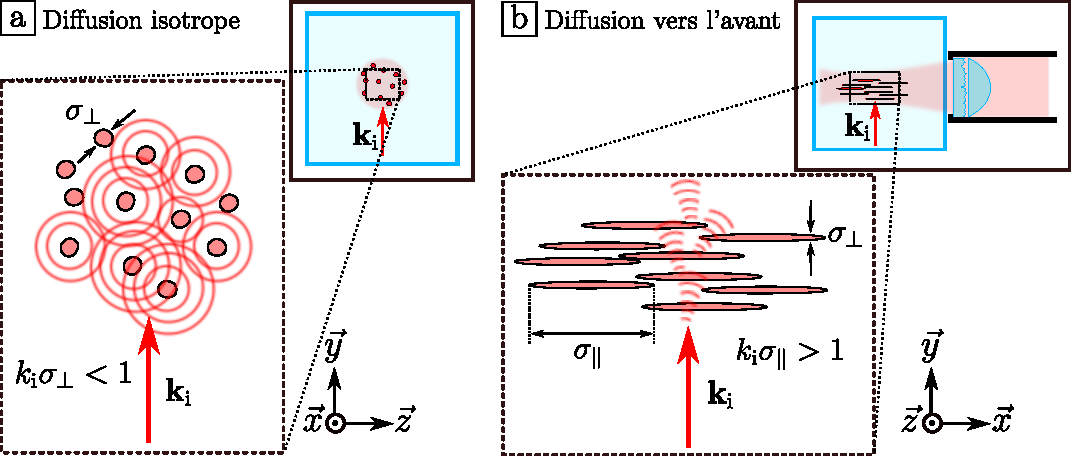
\includegraphics[width=\textwidth]{Fig/TauS_PRL/desordre_2D.pdf}
\caption{\textbf{Dynamique quasi-2D dans un \speckle .} Les grains de \speckle\ étant étendus selon la direction longitudinale, on peut trouver une configuration pour laquelle $k_{\mathrm{i}}\sigmal>1$, impliquant que la diffusion selon la direction $\vec{x}$ se fera essentiellement vers l'avant, et que $k_{\mathrm{i}}\sigmap<1$, impliquant une diffusion isotrope suivant les directions $\vec{y}$ et $\vec{z}$. De cette manière, on obtient une dynamique de diffusion quasi-2D, sans confiner le mouvement des atomes.}
\label{fig:desordre_2D}
\end{figure}

Plus précisément, nous avons vu au cours du chapitre \ref{ch:Speckle} que les grains de \speckle\ ne sont pas isotropes et possèdent deux tailles caractéristiques $\sigmap$ suivant les directions transverses et $\sigmal$ selon la direction longitudinale. Il est donc possible de se placer dans une situation où la diffusion est isotrope dans le plan transverse ($k_{\mathrm{i}}\sigmap<1$) tandis que celle-ci se déroule majoritairement vers l'avant selon l'axe optique ($k_{\mathrm{i}}\sigmal>1$). Pour des temps de propagation dans le désordre de l'ordre de quelques collisions élastiques, la dynamique de la diffusion sera essentiellement bidimensionnelle\footnote{Avec nos paramètres expérimentaux usuels $k_{\mathrm{i}}\sim\SI{1}{\micro\metre^{-1}}$ et $\sigmal/2\sim\SI{2}{\micro\metre}$, il faut environ $N=(\pi k_{\mathrm{i}} \sigmal)^2 \sim 150$ collisions pour que la diffusion devienne isotrope \citep{denechaud2018vers}.}, sans devoir confiner le mouvement des atomes.


\subsection{Temps de diffusion élastique dans le régime de Born}
\label{sc:taus_born}
Dans le régime de diffusion quasi-2D, on peut calculer $\taus^{\mathrm{Born}}$ à l'aide de la fonction de corrélation bidimensionnelle \ref{eq:correlation_2D_normalisee} que l'on peut réécrire sous la forme
\begin{equation}
C(\Delta \mathbf{r}_\perp)=\VR^2 \: e^{-\Delta\mathbf{r}_\perp^2/\sigmap^2}
\label{eq:correlation_2D_taus}
\end{equation}
afin de tenir compte de l'amplitude du désordre. Le passage à la limite continue de la règle d'or de Fermi \ref{eq:fermi_taus} permet de transformer la somme discrète sur les états finaux $\etat{\mathbf{k}'}$ en une intégrale:
\begin{equation}
\frac{1}{\taus^{\mathrm{Born}}}=\frac{2\pi}{\hb} \int{\frac{\diff^2 \mathbf{k}'}{(2\pi)^2} \: \widetilde{C}(\mathbf{k}'-\mathbf{k}_{\mathrm{i}}) \: \delta\left(\frac{\hb^2 k'^2}{2m}-\frac{\hb^2k_{\mathrm{i}}^2}{2m}\right)} \text{ .}
\label{eq:fermi_taus_continue}
\end{equation}

En injectant l'équation \ref{eq:correlation_2D_taus} dans la règle d'or de Fermi \ref{eq:fermi_taus_continue}, on peut ainsi obtenir une expression analytique dans le régime de diffusion quasi-2D \citep{shapiro2012cold}:
\begin{equation}
\frac{1}{\taus^{\mathrm{Born}} }=\frac{\pi}{\hb} \frac{\VR^2}{\ER} \: e^{- k_{\mathrm{i}}^2 \sigmap^2 /2} \: \mathrm{I_0}(k_{\mathrm{i}}^2 \sigmap^2 /2) \text{ ,}
\label{eq:taus_born_2D}
\end{equation}
où $\mathrm{I_0}$ est la fonction de Bessel modifiée d'ordre 0. Nous avons de plus fait apparaître l'énergie de corrélation $\ER$ dont l'expression se réduit à $\ER=\hb^2/m\sigmap^2\sim\SI{466}{\hertz}$ dans le cas d'un désordre bidimensionnel.

Il apparaît donc que le temps de diffusion élastique dépend d'une manière simple de l'amplitude du désordre $\VR$: $\taus^{\mathrm{Born}} \propto 1/\VR^2$. De manière plus générale, on peut définir un temps de diffusion élastique renormalisé $\tilde{\tau}_{\mathrm{s}}^{\mathrm{Born}}$ tel que
\begin{equation}
\taus^{\mathrm{Born}} (k_{\mathrm{i}},\VR)=\frac{\hb\ER}{\pi \VR^2} \tilde{\tau}_{\mathrm{s}}^{\mathrm{Born}} (k_{\mathrm{i}}) \text{ ,}
\end{equation}
qui est indépendant de $\VR$, dont le comportement est illustré en rouge sur la figure \ref{fig:prediction_taus_born}.

La formule \ref{eq:taus_born_2D} permet d'obtenir une expression approchée dans la limite de diffusion isotrope $k_{\mathrm{i}}\sigmap\ll 1$. On montre ainsi que le temps de diffusion devient indépendant de l'énergie initiale de l'onde et tend vers une constante \citep{richard2015propagation}:
\begin{equation}
\taus^{\mathrm{Born}} = \frac{\hb \ER}{\pi \VR^2}\quad \text{soit} \quad \tilde{\tau}_{\mathrm{s}}^{\mathrm{Born}}=1 \text{ .}
\end{equation}
De même, il est possible d'obtenir une expression simple du temps de diffusion élastique dans le régime de diffusion vers l'avant, pour lequel une dépendance en $k_{\mathrm{i}}$ est attendue étant donné que la diffusion se passe essentiellement dans la direction initiale de l'onde. On montre ainsi que dans le régime $k_{\mathrm{i}} \sigmap \gg 1$, le temps de diffusion élastique  dépend linéairement de l'impulsion initiale $\taus\propto k_{\mathrm{i}}\sigmap$ \citep{richard2015propagation}:
\begin{equation}
\taus^{\mathrm{Born}}=\frac{\hb\ER}{\VR^2\sqrt{\pi}} k_{\mathrm{i}} \sigmap \quad \text{soit} \quad \tilde{\tau}_{\mathrm{s}}^{\mathrm{Born}} = \sqrt{\pi} k_{\mathrm{i}} \sigmap \text{ ,}
\end{equation}
représenté en vert sur la figure \ref{fig:prediction_taus_born}.

\begin{figure}
\centering
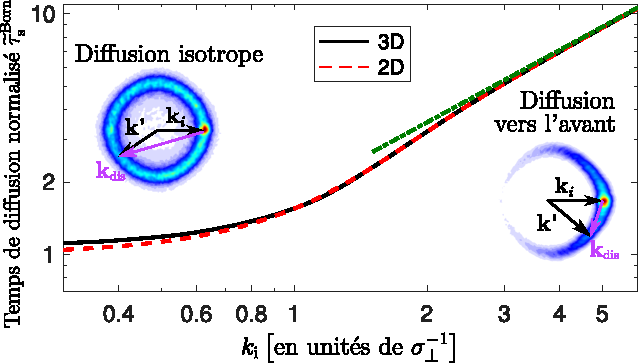
\includegraphics[scale=1]{Fig/TauS_PRL/prediction_taus_born.pdf}
\caption{\textbf{Prédiction de l'approximation de Born.} Le temps de diffusion élastique renormalisé $\tilde{\tau}_{\mathrm{s}}^{\mathrm{Born}}$ prédit par l'approximation de Born \ref{eq:taus_born_2D} est tracé en fonction de l'impulsion initiale de l'onde en pointillés rouges pour une configuration bidimensionnelle représentée par la fonction de corrélation \ref{eq:correlation_2D_taus}. Cette prédiction en configuration 2D est très proche de la configuration 3D représentée en noir calculée à l'aide la fonction de corrélation \ref{eq:correlation_3D_paraxial_effectif}. La limite asymptotique $\tilde{\tau}_{\mathrm{s}}^{\mathrm{Born}} \sim \sqrt{\pi} k_{\mathrm{i}} \sigmap$ est représentée en vert. Les illustrations des distributions de vitesses pour la diffusion isotrope ($k_{\mathrm{i}} \sigmap<1$) et la diffusion vers l'avant ($k_{\mathrm{i}} \sigmap>1$) correspondent à des images expérimentales.}
\label{fig:prediction_taus_born}
\end{figure}

Notons que d'éventuels effets tridimensionnels sont susceptibles de se manifester dans la limite de diffusion isotrope $k_{\mathrm{i}}\sigmap \ll 1$\footnote{Dans le cas à trois dimensions, $\taus^{\mathrm{Born}}$ tend aussi vers une constante pour de faibles impulsions initiales en raison de l'absence de limite de bruit blanc pour un \speckle . En effet, un \speckle\ possède une corrélation de portée infinie selon la direction longitudinale en raison de la propagation de la lumière \citep{goodman2007speckle}. Dans le cas d'une limite de bruit blanc et donc de corrélation de portée finie, le temps de diffusion élastique diverge en $1/k_{\mathrm{i}}$ dans la limite des faibles impulsions, que l'on peut reformuler comme $\ls\rightarrow\mathrm{cste}$. }. Il est possible d'estimer le temps de diffusion élastique dans une configuration 3D à l'aide de la fonction de corrélation \ref{eq:correlation_3D_paraxial_effectif} du modèle paraxial effectif. La prédiction de Born de notre configuration tridimensionnelle est représentée en noir sur la figure \ref{fig:prediction_taus_born} et ne montre qu'une légère déviation par rapport au cas bidimensionnel \ref{eq:taus_born_2D} pour les faibles impulsions initiales. Dans la suite, nous nous contenterons donc de décrire nos résultats à l'aide de la prédiction de l'équation \ref{eq:taus_born_2D}.


Le domaine de validité de l'approximation de Born peut être estimée d'une manière intuitive. En effet, le fait que l'état initial $\etat{\mathbf{k}_{\mathrm{i}}}$ possède un temps de vie $\taus^{\mathrm{Born}}$ fini se traduit par un élargissement de la distribution d'énergie de cet état dans le désordre de l'ordre de 
\begin{equation}
\Delta E= \hb/\taus^{\mathrm{Born}}\propto \frac{\VR^2}{\ER} \text{ .}
\end{equation} 
Pour valider l'approche perturbative, cette largeur doit être petite devant l'énergie initiale de l'onde $E_{\mathrm{k}_i}=\hb^2 k_{\mathrm{i}}^2 /2m$. La condition de désordre perturbatif s'écrit alors \citep{kuhn2007coherent}
\begin{equation}
E_{\mathrm{k}_i}\gg \frac{\VR^2}{\ER} \text{ .}
\label{eq:critere_kuhn}
\end{equation}

En comparant l'amplitude du désordre à son énergie de corrélation, il est possible de satisfaire la condition de désordre perturbatif tout en faisant apparaître deux régimes de désordre:
\begin{itemize}
\item[\textendash] Supposons que l'amplitude du désordre soit supérieure à l'énergie de corrélation $\VR\gg\ER$. La condition de désordre perturbatif impose que l'énergie de l'onde soit très grande devant l'amplitude du désordre, et donc que celle-ci ne soit que faiblement perturbée par le désordre. Ainsi, la trajectoire de la particule est essentiellement classique\footnote{Pour $\VR\gg\ER$, les fluctuations du potentiel peuvent supporter des états liés. Dans la limite $\VR/\ER\rightarrow\infty$, ces états liés forment un continuum pour lequel le mouvement des particules est classique.}. Dans cette limite, on parle de \emph{désordre classique}.
\item[\textendash] Supposons que l'énergie de corrélation du désordre soit supérieure à son amplitude $\ER\gg\VR$. Il est possible de satisfaire la condition de désordre perturbatif en ayant $E_{\mathrm{k}_i}<\VR$, c'est-à-dire que la propagation de la particule se fait par effet tunnel au travers des fluctuations de potentiel. Plus particulièrement, l'amplitude du potentiel est renormalisée par l'effet tunnel, l'amplitude effective du potentiel étant $\VR^2/\ER$. On parle alors de \emph{désordre quantique}.
\end{itemize}
Le rapport entre l'amplitude du désordre et son énergie de corrélation joue donc un rôle fondamental dans la description de la physique du désordre\footnote{Il s'agit de la raison pour laquelle la figure \ref{fig:seuil_mobilite_delande} décrivant l'évolution du seuil de mobilité avec l'amplitude du potentiel est tracée en fonction de cette quantité. En particulier, la physique de la localisation peut être assimilée à un piégeage classique dans la limite $\VR/\ER\rightarrow\infty$ (le seuil de mobilité converge vers le seuil de percolation classique), tandis que la localisation d'Anderson d'ondes de matière est de nature purement quantique lorsque $\VR<\ER$.}. 

Notons qu'il est aussi possible d'écrire la condition de désordre faible sous la forme $k_{\mathrm{i}}\ls^{\mathrm{Born}}\gg 1$, identifiable au critère de Ioffe-Regel\footnote{Notons que ce critère coïncide avec celui $E_{\mathrm{k}}\gg \VR^2/\ER$ utilisé par \citep{kuhn2007coherent} dans le régime de diffusion isotrope. Dans le régime de diffusion vers l'avant, ces deux critères dévient de manière significative.}. Une analyse du temps de diffusion élastique en fonction des paramètres expérimentaux $\VR$ et $k_{\mathrm{i}}$ nous permet alors de tester la validité de ce critère en étudiant la transition entre les régimes de diffusion faible et de diffusion forte, que l'on pourra confronter à celle du critère \ref{eq:critere_kuhn} utilisé par \citep{kuhn2007coherent}.




\section{Mesure du temps de diffusion élastique}
Les différentes étapes expérimentales menant à l'obtention d'une onde de matière plane ainsi que les différentes configurations magnétiques utilisables ont pu être présentées dans les chapitres \ref{ch:BEC_manip} et \ref{ch:new_exp}. 

Dans cette partie, nous allons présenter le protocole expérimental utilisé pour mesurer le temps de diffusion élastique ainsi que la manière dont celui-ci a été extrait des données expérimentales. Rappelons que ces données ont obtenues en 2015 lors de la thèse de Jérémie Richard \citep{richard2015propagation}, mais que celles-ci ont été entièrement retraitées au cours de ma thèse. 

\subsection{Procédure expérimentale}
La séquence de génération d'un condensat de Bose-Einstein correspond à celle décrite au cours du chapitre \ref{ch:BEC_manip}. On obtient ainsi un nuage dégénéré d'environ $10^5$ atomes de \isotope[87]{Rb} interagissant faiblement dans un piège optique fortement décomprimé après évaporation. Ce nuage est polarisé dans le sous-état Zeeman $\etatF{2}{-2}$ et suspendu contre la gravité à l'aide de la lévitation magnétique qui est anti-piégeante. 

Dans un second temps, le nuage est refroidi davantage à l'aide du refroidissement par delta-kick présenté en section \ref{sc:chambre_science}, permettant d'obtenir en dispersion en impulsion de $\Delta k=\SI{0.15}{\micro\metre^{-1}}$, soit une température équivalente de $T\sim\SI{150}{\pico\kelvin}$. Enfin, une impulsion initiale $\mathbf{k}_{\mathrm{i}}$ selon la direction $\vec{y}$ est conférée au nuage à l'aide d'un gradient magnétique. Cette impulsion initiale varie ainsi de \SI{1}{\micro\metre^{-1}} à \SI{20}{\micro\metre^{-1}} en modifiant la durée d'application du gradient magnétique. Le nuage peut ainsi être assimilé à une onde plane $\etat{\mathbf{k}_{\mathrm{i}}}$ d'impulsion et d'énergie bien définies.


Le désordre est ensuite brusquement\footnote{Le temps d'allumage du faisceau \speckle\ est d'environ \SI{50}{\micro\second}, limité par la bande-passante de l'atténuateur variable de la radio-fréquence envoyée dans le modulateur acousto-optique utilisé pour l'asservissement de puissance.} allumé sur les atomes à $t=\SI{0}{\second}$. Ce désordre est réalisé à l'aide du champ de \speckle\ décrit au cours du chapitre \ref{ch:Speckle}, dont la différence entre les longueurs de corrélation $\sigmap$ et $\sigmal$ permet de considérer le \speckle\ comme un désordre quasi-2D dans le plan $(y-z)$ du repère de l'expérience. Le faisceau \speckle\ est accordable autour de la transition $D_2$ du \isotope[87]{Rb} à \SI{780}{\nano\metre}, permettant de réaliser un désordre qui soit attractif ou répulsif, comme expliqué dans la section \ref{sc:propriete_potentiel_speckle}. Le désaccord utilisé $|\delta|/2\pi\sim\SI{1}{\tera\hertz}$ est suffisamment faible pour que les propriétés du potentiel soient identiques entre les configurations attractive et répulsive, mais il est de plus suffisamment grand pour que le potentiel soit conservatif\footnote{Le taux d'émission spontanée est au plus de \SI{0.1}{\second^{-1}}.}. L'amplitude du désordre $|\VR|$ est fixée en contrôlant la puissance du faisceau \speckle , $|\VR|/h$ pouvant ainsi aller de \SI{39}{\hertz} à \SI{3.88}{\kilo\hertz}. 

Le temps de diffusion élastique pouvant être extrait de la déplétion de l'état initial $\etat{\mathbf{k}_{\mathrm{i}}}$ d'après l'équation \ref{eq:decroissance_exponentielle_taus}, l'approche naturelle à son étude consiste donc à suivre l'évolution de la distribution d'impulsion du nuage en fonction du temps de propagation $t$ dans le désordre. Celle-ci est obtenue à l'aide d'un très grand temps de vol après extinction du désordre: après une longue expansion balistique, la position des atomes ne dépend plus de la taille initiale du nuage et n'est due qu'à leur vitesse. Ainsi, des temps de vol allant jusqu'à \SI{300}{\milli\second} peuvent être utilisés grâce à la lévitation magnétique, permettant d'obtenir une résolution d'impulsion de $\Delta k_{\mathrm{res}}=\SI{0.2}{\micro\metre^{-1}}$\footnote{Cette résolution est supérieure à la dispersion initiale d'impulsion en raison de la taille du nuage, d'environ \SI{30}{\micro\metre}, et du temps fini d'expansion.}. Enfin, la densité atomique est mesurée dans le plan $(\mathbf{k}_{\mathrm{y}}-\mathbf{k}_{\mathrm{z}})$ (le plan $(y-z)$ du repère de l'expérience) à l'aide d'une imagerie par fluorescence.

\subsection{Extraction du temps de diffusion élastique}
\label{sc:traitement_donnees_extraction_taus}

L'évolution temporelle de la population de l'état initial $n(\mathbf{k}_{\mathrm{i}},t)$ est obtenue à l'aide des images expérimentales de la distribution dans l'espace des impulsions. La figure \ref{fig:extraction_taus}.a représente la distribution expérimentale d'impulsion $n(\mathbf{k},t)$ pour les paramètres $k_{\mathrm{i}}=2.31\sigmap^{-1}$ et $\VR/h=\SI{-104}{\hertz}$, pour des temps de propagation dans le désordre $t=\SI{0}{\milli\second}$ (état initial) et $t=\SI{17.5}{\milli\second}$. 

Après propagation dans le désordre, les atomes initialement dans l'état $\etat{\mathbf{k}_{\mathrm{i}}}$ sont diffusés dans les états $\etat{\mathbf{k}'}$. On remarque que les atomes diffusés se répartissent selon un anneau tel que $|\mathbf{k}'|=|\mathbf{k}_{\mathrm{i}}|$, témoignant du caractère élastique de la diffusion dans le désordre. Néanmoins, cet anneau admet une largeur finie $\Delta k_{\mathrm{incoh}}$ en raison de l'élargissement en énergie lié au temps de vie fini de l'onde plane initiale dans le désordre. On peut ainsi montrer que $\Delta k_{\mathrm{incoh}}\sim 2/\ls$ \citep{cherroret2012coherent}.

\begin{figure}
\centering
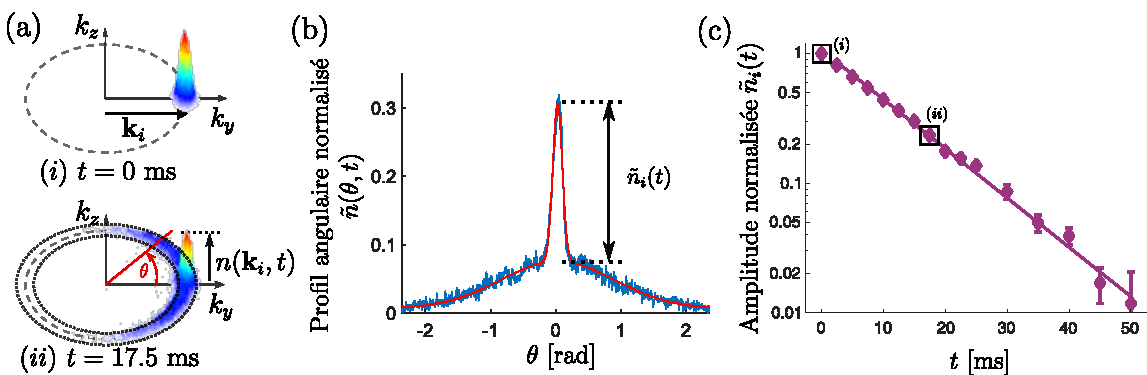
\includegraphics[width=\textwidth]{Fig/TauS_PRL/extraction_taus.pdf}
\caption{\textbf{Extraction du temps de diffusion élastique.} La procédure d'extraction du temps de diffusion élastique est illustrée pour les paramètres expérimentaux $\VR/h=\SI{-104}{\hertz}$ et $k_{\mathrm{i}}=2.31\sigmap^{-1}$. \textbf{a:} Distributions expérimentales d'impulsion $n(\mathbf{k},t)$ de l'état initial ($t=0$) et après propagation dans le désordre ($t=\SI{17.5}{\milli\second}$). Une intégration radiale (suivant la ligne rouge et délimitée par les lignes pointillées noires) permet d'obtenir le profil angulaire. \textbf{b:} Profil angulaire normalisé $\tilde{n}(\theta,t)$ (en bleu), ajusté par une structure bimodale (en rouge). L'amplitude de l'état initial est extraite de la partie gaussienne fine, tandis que la partie gaussienne large représente le peuplement d'autres états par des atomes diffusés. \textbf{c:} Décroissance de l'amplitude normalisée $\tilde{n}_{\mathrm{i}}(t)$, tracée en échelle semi-logarithmique. Celle-ci est ajustée par une exponentielle, permettant d'extraire $\taus=12.0\pm\SI{0.3}{\milli\second}$. Les points encadrés $(i)$ et $(ii)$ sont issus des distributions expérimentales d'impulsion présentées figure \textbf{a}.}
\label{fig:extraction_taus}
\end{figure}

La détermination de $\taus$ repose sur la succession de trois étapes de traitement de données illustrées figure \ref{fig:extraction_taus}. Dans un premier temps, la densité atomique $n(\mathbf{k},t)$ dans le plan $(\mathbf{k}_{\mathrm{y}}-\mathbf{k}_{\mathrm{z}})$ est intégrée radialement afin d'obtenir le profil angulaire $n(\theta,t)$. Les bornes d'intégration correspondent  à deux fois la demi-largeur de la distribution d'impulsion initiale $n(\mathbf{k},0)$ (figure \ref{fig:extraction_taus}.a). Le profil angulaire est ensuite normalisé par sa valeur à l'origine $\theta=0$ et $t=0$, $\tilde{n}(\theta,t)= n(\theta,t)/n(0,0)$. Le profil angulaire normalisé obtenu est le résultat de la somme de deux contributions, une distribution fine correspondant à la distribution initiale non diffusée $\tilde{n}_{\mathrm{i}}(\theta,t)$, et une seconde structure $\tilde{n}_{\mathrm{b}}(\theta,t)$ plus large identifiée aux atomes diffusés dans les états $\etat{\mathbf{k}'}$ (figure \ref{fig:extraction_taus}.b). 

Dans un second temps, le profil angulaire normalisé est ajusté à l'aide de la somme d'une gaussienne large, représentant le fond diffusé $\tilde{n}_{\mathrm{b}}(\theta,t)$, et d'une gaussienne étroite décrivant la distribution initiale $\tilde{n}_{\mathrm{i}}(\theta,t)$\footnote{Le profil du paquet d'onde ne correspond plus à un profil de Thomas-Fermi en raison de l'étape de refroidissement par delta-kick. Il a été observé que celui-ci était mieux décrit à l'aide d'une fonction gaussienne.}. On obtient ainsi l'amplitude normalisée $\tilde{n}_{\mathrm{i}}(t)=\tilde{n}_{\mathrm{i}}(0,t)$, dont les barres d'erreur sont estimées à l'aide des incertitudes expérimentales et des déviations de l'ajustement bimodal. 

Enfin, l'évolution temporelle de l'amplitude du pic initial $\tilde{n}_{\mathrm{i}}(t)$, suivie sur deux décades, est ajustée par une décroissance exponentielle\footnote{Comme nous le verrons dans le chapitre \ref{ch:TauS_NJP}, il est attendu que dans un régime de très fort désordre la décroissance de l'état initial ne soit plus exponentielle \citep{trappe2015semiclassical}, cependant nous n'avons pas observé de déviation expérimentale importante à la décroissance exponentielle.} \ref{eq:decroissance_exponentielle_taus} de temps de vie $\taus$, valant $12.0\pm\SI{0.3}{\milli\second}$ dans le cas de la figure \ref{fig:extraction_taus}.c. Les incertitudes associées sont estimées à partir des barres d'erreurs de l'amplitude du pic de la distribution initiale et de la déviation de l'ajustement exponentiel. 




\subsection{Cartographie du temps de diffusion élastique}

La procédure de mesure du temps de diffusion élastique décrite dans les deux sections précédentes est répétée pour une large gamme de paramètres expérimentaux $|\VR|$ et $k_{\mathrm{i}}$, ainsi que pour des désordres désaccordés vers le rouge (désordres attractifs) et vers le bleu (désordres répulsifs) décrits dans le chapitre \ref{ch:Speckle}. En balayant l'impulsion initial $k_{\mathrm{i}}$ sur un ordre de grandeur et l'amplitude du désordre $|\VR|$ sur deux ordres de grandeur, nous avons pu observer des variations de $\taus$ allant de \SI{40}{\micro\second} à \SI{100}{\milli\second}, représentant près de quatre ordres de grandeur. 

L'ensemble des valeurs mesurées peut être retrouvé figure \ref{fig:donnees_taus_prl}, dans laquelle le temps mesuré $\taus$ est tracé en fonction de l'impulsion initiale $k_{\mathrm{i}}$ en échelle logarithmique. Les différentes couleurs correspondent aux différentes amplitudes de désordre utilisées. Les données expérimentales (points) sont comparées à la prédiction de Born \ref{eq:taus_born_2D} (lignes pointillées) ainsi qu'à des simulations numériques (lignes continues). 

\begin{figure}
\centering
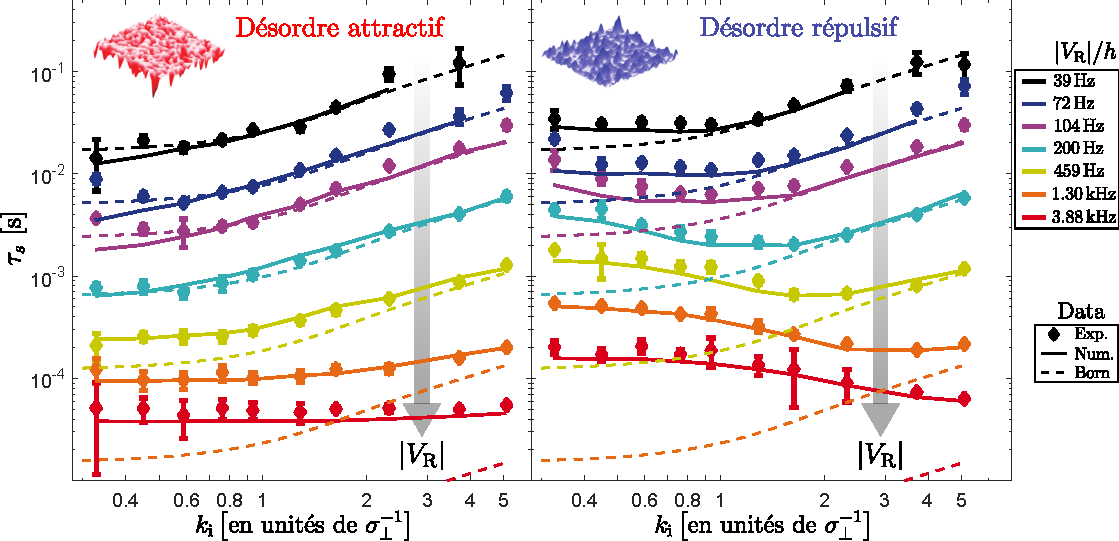
\includegraphics[width=\textwidth]{Fig/TauS_PRL/donnees_taus_prl.pdf}
\caption{\textbf{Cartographie du temps de diffusion élastique en fonction des paramètres expérimentaux.} Le temps de diffusion élastique est tracé en fonction de l'impulsion initiale pour différentes amplitude du désordre (différentes couleurs) ainsi que pour des désordres attractifs (cadre de gauche) et des désordres répulsifs (cadre de droite). Les données expérimentales (points) sont comparées à des données numériques \textit{ab-initio} (lignes continues) ainsi qu'à la prédiction bidimensionnelle de Born \ref{eq:taus_born_2D} (lignes pointillées).}
\label{fig:donnees_taus_prl}
\end{figure}

Ces simulations correspondent à la résolution numérique en deux dimensions de l'équation de Schrödinger décrivant l'évolution d'un paquet d'onde gaussien dans un désordre dont les propriétés vérifient la distribution de potentiel \ref{eq:distribution_potentiel_speckle} ainsi que la fonction de corrélation \ref{eq:correlation_2D_taus}. La résolution numérique s'appuie sur une méthode de différences finies ainsi que l'utilisation de conditions aux limites absorbantes. La distribution d'impulsion est obtenue par transformation de Fourier de la fonction d'onde avant d'être moyennée sur 14 réalisations du désordre\footnote{Nous avons déterminé que moyenner la distribution d'impulsion sur 14 réalisations du désordre permettait d'atteindre la convergence vers la distribution moyenne d'impulsion.}. La détermination du temps de diffusion élastique est finalement réalisée de la même manière que pour les données expérimentales, explicitée section \ref{sc:traitement_donnees_extraction_taus}.

La figure \ref{fig:donnees_taus_prl} témoigne d'un accord remarquable entre les données expérimentales et les données numériques sur l'ensemble des paramètres expérimentaux et confirme ainsi le caractère quasi-2D de notre système. Néanmoins, des petites déviations sont observées dans la région d'impulsion et de désordre faibles (région en haut à gauche), que l'on peut attribuer à deux contributions. En effet, la zone d'impulsions faibles est susceptible de témoigner d'effets tridimensionnels. De plus, la résolution finie de la distribution d'impulsion $\Delta k_{\mathrm{res}}$ engendre des difficultés expérimentales pour déterminer précisément $\taus$.

L'excellent accord entre les données expérimentales et les données numériques nous permet de calibrer l'amplitude du désordre $\VR$ utilisé expérimentalement. Notamment, celle-ci est estimée à l'aide de mesures photométriques de la puissance du faisceau utilisé, sujettes à des erreurs systématiques de quelques dizaines de pourcents, qu'il est possible de corriger à l'aide d'un facteur de calibration $\alpha$. En minimisant les différences entre les données numériques et expérimentales pour l'impulsion $k_{\mathrm{i}}=0.74 \sigmap^{-1}$, on détermine ainsi le facteur de calibration $\alpha=1.29\pm0.02$.




\section{Comportement du temps de diffusion élastique}
\label{sc:comportement_taus}
Nous avons vu dans la section précédente comment nous avons mesuré le temps de diffusion élastique pour de larges gammes de paramètres $k_{\mathrm{i}}$ et $\VR$. À présent, nous allons voir comment ces données se comparent à la théorie de Born. Plus précisément, c'est la comparaison à la prédiction de Born qui nous permettra de différencier les régimes de diffusion faible et de diffusion forte. En particulier, nous allons illustrer l'influence de la distribution de potentiel sur la transition entre ces régimes, que nous confronterons au critère de désordre faible $k_{\mathrm{i}}\ls^{\mathrm{Born}}\sim 1$.

\subsection{Régime de Born}
Comme nous l'avons dit ci-dessus, les données expérimentales et numériques sont comparées aux prédictions du régime de Born dans la figure \ref{fig:donnees_taus_prl}. Remarquons que la prédiction théorique du régime de Born, représentée par les lignes pointillées, est simplement translatée verticalement en changeant l'amplitude du désordre $|\VR|$ en vertu de la loi d'échelle $\taus^{\mathrm{Born}} \propto 1/|\VR|^2$. De plus, celle-ci est identique pour les désordres attractif et répulsif étant donné que la prédiction \ref{eq:fermi_taus} ne dépend pas de la distribution de potentiel, mais uniquement du spectre des fréquences spatiales du désordre $\widetilde{C}(\mathbf{k}_{\mathrm{dis}})$. 

De manière générale, $\taus^{\mathrm{Born}}$ montre un bon accord avec les données dans le régime de diffusion faible, c'est à dire la région de désordre faible (petits $|\VR|$) et d'impulsion importante (grands $k_{\mathrm{i}}$). On observe ainsi les comportements de diffusion isotrope ($k_{\mathrm{i}}\sigmap<1$) et de diffusion vers l'avant ($k_{\mathrm{i}}\sigmap>1$), notamment pour la courbe noire de plus faible désordre $|\VR|/h=\SI{39}{\hertz}$. 

Cependant, l'augmentation de l'amplitude du désordre ou la diminution de l'impulsion initiale mènent à de fortes déviations à la prédiction de théorique de Born, obtenue dans le cadre de la théorie des perturbations. %L'augmentation de la force de la diffusion montre alors la limite de l'approche de Born.


\subsection{Déviations au régime de Born}
\label{sc:deviation_regime_born}
En dehors du régime dans lequel l'approximation de Born permet de décrire quantitativement nos données, nous observons de larges déviations entre les désordres attractifs et répulsifs. Cette signature de l'influence de la distribution de potentiel $\mathcal{P}(V)$ montre l'insuffisance de l'approximation de Born pour décrire le régime de diffusion forte.

Une représentation visuelle des déviations observées à l'approximation de Born est proposée figure \ref{fig:map_deviations_born}, où le rapport $\taus/\taus^{\mathrm{Born}}$ est tracé en échelle logarithmique en fausses couleurs en fonction des paramètres expérimentaux $k_{\mathrm{i}}$ et $|\VR|$ pour les différents désordres considérés.  Afin d'exposer le rôle fondamental de la distribution de potentiel, cette étude est de plus étendue au cas d'un désordre gaussien\footnote{L'extension de l'étude au potentiel gaussien n'a pu être réalisée que numériquement. Celui-ci possède la même fonction de corrélation \ref{eq:correlation_2D_taus} que les potentiels de type \speckle . La génération expérimentale d'un tel potentiel peut être envisagée en réalisant l'interférence entre un \speckle\ et une onde plane intense, ou encore à l'aide d'un modulateur spatial de lumière.} dont la distribution de potentiel est donnée par
\begin{equation}
\mathcal{P}(V)=\frac{1}{\sqrt{2\pi} \VR} e^{-V^2/2\VR^2} \text{ .}
\end{equation}

\begin{figure}
\centering
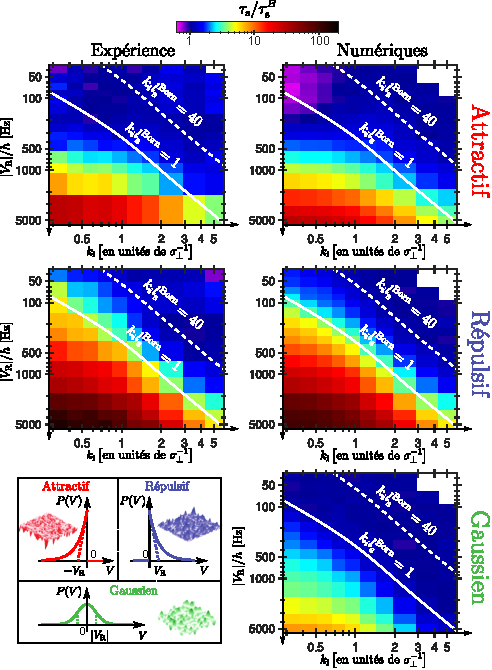
\includegraphics[width=0.95\textwidth]{Fig/TauS_PRL/map_deviations_born.pdf}
\caption{\textbf{Cartographie des déviations au régime de Born.} Le rapport $\taus/\taus^{\mathrm{Born}}$ est tracé en échelle logarithmique en fausses couleurs en fonction des paramètres expérimentaux $k_{\mathrm{i}}$ et $|\VR|$. Les données expérimentales (colonne de gauche) et numériques (colonne de droite) sont tracées pour les désordres attractifs (première ligne), répulsifs (deuxième ligne) ainsi que pour un désordre gaussien (figure en bas à droite) ayant la même fonction de corrélation \ref{eq:correlation_2D_taus} que les désordres \speckle . Les distributions $\mathcal{P}(V)$ des potentiels sont représentées dans la figure en bas à gauche. Les courbes blanches correspondent aux critères phénoménologiques de désordre faible $k_{\mathrm{i}}\ls^{\mathrm{Bron}}=1$ (ligne continue) et $k_{\mathrm{i}}\ls^{\mathrm{Born}}=40$ (ligne pointillée). }
\label{fig:map_deviations_born}
\end{figure}

Le parties bleues des cartes du temps de diffusion élastique de la figure \ref{fig:map_deviations_born} représentent le régime pour lequel $\taus/\taus^{\mathrm{Born}}\sim 1$. On observe que ces régions où l'estimation de Born est quantitativement correcte se trouvent dans la zone de désordres faibles et d'impulsions importantes, comme attendu. La région de fort désordre et d'impulsion faible témoigne en revanche de déviations extrêmes, où des déviations de deux ordres de grandeurs ont pu êtres observées.

Les déviations mesurées à l'approximation perturbative permettent ainsi de révéler la forte influence de la distribution de potentiel sur le régime de diffusion forte, ainsi que sur la transition entre le régime de Born et le régime de diffusion forte. Notamment, le critère de validité de l'approximation de Born communément utilisé $k_{\mathrm{i}}\ls^{\mathrm{Born}}=1$ est tracé en ligne blanche continue et semble reproduire remarquablement la zone de transition entre le régime de Born et le régime de diffusion forte. Plus particulièrement, nous avons observé que la ligne $k_{\mathrm{i}}\ls^{\mathrm{Born}}=1$ correspondait à une iso-déviation de 25\% dans le cas du désordre gaussien\footnote{Il s'agit de la ligne de niveau $\taus/\taus^{\mathrm{Born}}=1.25$ dans le cas du désordre gaussien.}. On vérifie ainsi la pertinence de ce critère pour localiser la transition entre régimes de diffusion faible et forte pour un désordre gaussien, largement utilisé.

Néanmoins, les déviations observées sont beaucoup plus marquées pour les désordres de type \speckle , montrant la désadaptation de ce critère à ce type de désordre. En effet, la ligne $k_{\mathrm{i}}\ls^{\mathrm{Born}}=1$ témoigne de déviations atteignant 250\% pour un \speckle\ attractif, et 400\% pour un \speckle\ répulsif. Il apparaît donc que la transition entre les régimes de diffusion faible et forte est déplacée vers des valeurs plus importantes de la quantité $k_{\mathrm{i}} \ls^{\mathrm{Born}}$, notamment, des déviations de 25\% mentionnées précédemment apparaissent dès $k_{\mathrm{i}} \ls^{\mathrm{Born}}=40$ (lignes blanches pointillées). La pertinence du critère communément utilisé $k_{\mathrm{i}} \ls^{\mathrm{Born}}\sim 1$ dépend donc de la nature du désordre utilisé.

La description du comportement du temps de diffusion élastique hors du régime de Born fait l'objet du chapitre \ref{ch:TauS_NJP}, mais nous pouvons néanmoins décrire brièvement la nature des déviations au régime de Born. La région des faibles désordres correspond à celle où l'approximation de Born est susceptible d'être valide. Cependant, pour des impulsions faibles, l'énergie de l'onde initiale n'est pas suffisamment grande pour que seul le premier ordre de la théorie des perturbations puisse décrire correctement le temps de diffusion élastique. Notamment, l'ordre suivant de la théorie des perturbations, en $1/\VR^3$, permet d'expliquer l'asymétrie du comportement entre les trois désordre considérés dans la région de faibles désordre et impulsion.

La région de fort désordre sort naturellement du cadre de la théorie perturbative de Born. Il s'agit de la région pour laquelle la distribution de potentiel joue un rôle capital, comme cela est illustré par la différence significative des déviations que l'on peut observer dans cette région pour les différents désordres. Nous verrons dans le chapitre suivant que dans ce régime, l'évolution temporelle de l'état initial est directement reliée à sa distribution d'énergie, donnée par la fonction spectrale $A(\mathbf{k}_{\mathrm{i}},E)$ et dont le profil est intimement relié à la distribution de potentiel.


\subsection{Déviation à la décroissance exponentielle}
La décroissance exponentielle de la population de l'état initial étant une prédiction du régime perturbatif de Born, des déviations à ce comportement exponentiel sont attendues dans le régime de diffusion forte. Si celles-ci n'ont pas pu être observées avec nos données expérimentales\footnote{La précision de nos mesures n'a permis de démontrer des déviations significatives au comportement exponentiel.}, nos simulations révèlent des signatures de la physique hors-Born dans les décroissances de l'état initial.

En particulier, un comportement \emph{universel} à temps court a pu être observé à l'aide de nos données numériques
\begin{equation}
\tilde{n}_{\mathrm{i}}(t)=1-\frac{\VR^2t^2}{\hb^2} \text{ ,}
\label{eq:depart_quadratique}
\end{equation}
valide pour les temps courts $t<\hb/\ER$. Si ce départ quadratique est attendu dans le régime classique\footnote{Celui-ci trouve son origine dans le comportement des fonctions spectrales dans le régime classique. Nous aborderons ce point dans le chapitre \ref{ch:TauS_NJP}.}, celui-ci est aussi observé dans le régime de Born, que nous allons à présenter détailler.

L'application de la règle d'or de Fermi \ref{eq:fermi_golden_rule} repose non seulement sur l'hypothèse de désordre perturbatif, mais aussi sur la considération de temps de couplage $t$ suffisamment longs pour résoudre les niveaux d'énergie du système. Notamment, le terme de conservation de l'énergie $\delta(E_{\mathrm{k}'} - E_{\mathrm{k}_i})$ correspond à la limite aux temps longs d'une fonction donnant la résolution en énergie du couplage \citep{grynberg2010introduction}:
\begin{equation}
g_{\mathrm{t}}(E_{\mathrm{k}'} - E_{\mathrm{k}_i}) = \frac{\sin^2((E_{\mathrm{k}'} - E_{\mathrm{k}_i})t/2\hb)}{((E_{\mathrm{k}'} - E_{\mathrm{k}_i})t/2\hb)^2} t^2 \quad \xrightarrow{t\to\infty} \quad \delta(E_{\mathrm{k}'} - E_{\mathrm{k}_i}) \text{ ,}
\end{equation}
dans le cas d'une perturbation constante.

Plus particulièrement, cette approximation de temps longs est valable lorsque le temps de couplage est grand devant le temps caractéristique donné par la largeur en énergie du continuum, $t\gg\hb/\ER$. En effet, le désordre possédant une fréquence spatiale de coupure $\sigmap^{-1}$, il s'ensuit un transfert d'énergie maximal de $\ER$ dans le cas de collisions inélastiques.

Néanmoins, dans la limite de temps courts $t<\hb/\ER$, la fonction de résolution en énergie du couplage précédente possède une largeur plus grande que celle du continuum adressé. De fait, ce dernier peut être considéré comme un état unique. Le couplage induit donc une oscillation de Rabi entre l'état initial et \emph{l'unique état} final, caractérisé par un départ quadratique de l'oscillation.

\begin{figure}
\centering
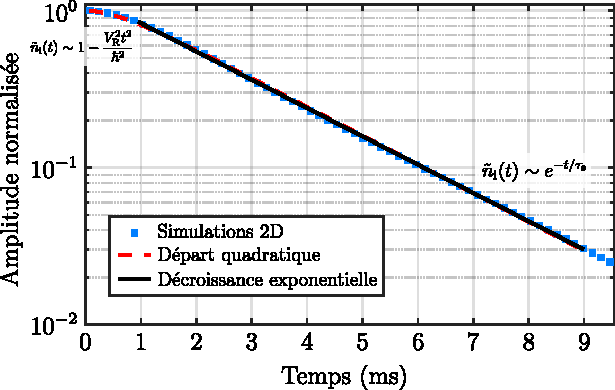
\includegraphics[width=0.75\textwidth]{Fig/TauS_PRL/depart_quadratique_taus.pdf}
\caption{\textbf{Départ quadratique de la décroissance de l'état initial.} Cette décroissance est issue de simulations numériques  pour un désordre de type \speckle\ avec comme paramètres $\VR=\SI{-104}{\hertz}$ et $k_{\mathrm{i}}=0.59\sigmap^{-1}$. Celle-ci fait apparaître le régime de temps courts pour lequel la décroissance est quadratique, suivi du régime de décroissance exponentielle. Les points bleus correspondent aux données, la ligne noire continue correspond à l'ajustement par une exponentielle, et la ligne pointillée rouge correspond à un ajustement donné par l'équation \ref{eq:depart_quadratique_total}. }
\label{fig:depart_quadratique_taus}
\end{figure}

La décroissance de l'état initial est donc composée de deux régimes comme illustré sur la figure \ref{fig:depart_quadratique_taus} pour les paramètres $\VR=\SI{-104}{\hertz}$ et $k_{\mathrm{i}}=0.59\sigmap^{-1}$. Un premier régime à temps court est caractérisé par une décroissance quadratique liée au début d'une oscillation de Rabi entre l'état initial et le continuum de largeur finie lui-même. Dans un second temps, le couplage est suffisamment long pour que la conservation de l'énergie soit satisfaite, la décroissance est alors exponentielle avec un temps de vie donné par la règle d'or de Fermi.

Ainsi, il est possible d'obtenir une expression de la décroissance à l'aide d'un modèle simple dans le régime de désordre faible \citep{grynberg2010introduction} permettant de décrire à la fois le départ quadratique observé et la décroissance exponentielle de l'état initial:
\begin{equation}
\tilde{n}_{\mathrm{i}}(t)=\left| e^{-t/\taus^{\mathrm{Born}}/2} \left(1+\frac{\hb}{2\ER\taus^{\mathrm{Born}}} \right) - \frac{\hb}{2\ER\taus^{\mathrm{Born}}} e^{-\ER t/\hb}\right|^2 \text{ ,}
\label{eq:depart_quadratique_total}
\end{equation}
dont le développement limité permet de retrouver le départ quadratique \ref{eq:depart_quadratique}. Cette forme est utilisée pour ajuster la décroissance numérique, et est représentée en pointillés rouges sur la figure \ref{fig:depart_quadratique_taus}. On remarque que celle-ci décrit correctement l'ensemble de la décroissance là où une décroissance exponentielle pure ne permet pas d'en reproduire le début. Cependant, cette approche de désordre de faible reste inadaptée à la description du régime de désordre fort.


\section{Conclusion}
